\section{Introdução}
%%%%%%%%%%%%%%%%%%%%%%%%%%%%%%%%%%%%%%%%%%%%%%%%%%%%%%%%%%%%%%%%%
\qquad A juventude foi ensinada que a missão de se tornarem adultos, o caminho de dignidade, segurança e independência é obter um emprego. \cite{book-11} \\
E o estágio uma ferramenta muito importante para qualquer iniciante de qualquer profissão de forma a ser transmitido conhecimentos adquiridos, que em certas profissões pode demorar até alguns anos para alcançar a categoria de oficial ou sénior.
\emptyline
O cidadão deve estar numa das situações contributiva abaixo descrito para ser considerado um trabalhador em regime legal. \\
\\
\begin{minipage}[t]{\linewidth}
	\begin{itemize}
		\setlength\itemsep{-0.3em}
		\item Trabalhador por conta de outrem
		\begin{itemize}
			\item Organização privada
			\item Organização pública
		\end{itemize}
		\item Trabalhadores independentes
		\newpage
		\item Trabalhador do serviço domestico
		\item Membros de órgãos estatuários
		\item Empresa
		\item Político
	\end{itemize}
\end{minipage}
\subsection{Trabalhador por conta de outrem}
\begin{figure}[H]
	%\centering
	\flushleft
	%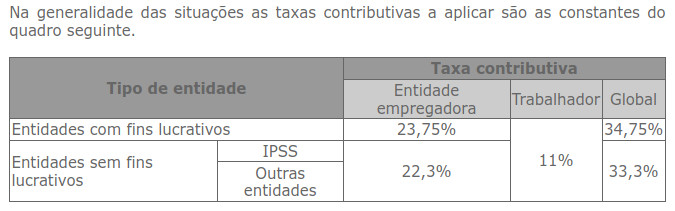
\includegraphics[width=.6\textwidth,left]{./image/SGS/Contribuicoes_1.jpg}
	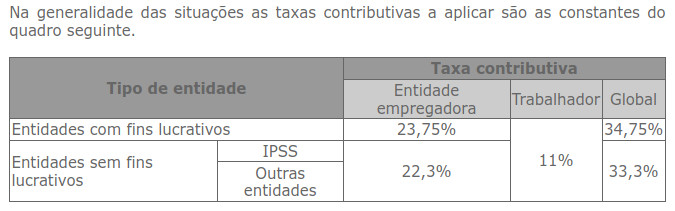
\includegraphics[scale=.5]{./image/SGS/Contribuicoes_1.jpg}
	\caption{Contribuições para SGS}
\end{figure}
\textbf{Exemplo:}
\newline
Vencimento de 1000Eur será descontado 11\% para a Segurança Social, ficando com $1000\times (1-0,11)=890Eur$ e a empresa desconta para o exemplo de 23,75\%, $1000\times 0,2375=237,5Eur$, ao todo será descontado $110+237,5=347,5Eur$, ou seja, todos os messes um trabalhador que ganhe 1000Eur desconta para a Segurança Social direto e indiretamente \textbf{347,5Eur}.
\emptyline
Na realidade o vencimento neste exemplo do cidadão devia ser de \textbf{1237,5Eur}, ou seja, é prejudicado nos seus descontos na quantia de 237,5Eur [23,75\%] pois não são considerados como pessoais. \\
A circulação deste capital passa despercebido e usado pelo estado para seus gastos, sendo o cidadão sua fonte, sem nenhum proveito, a não ser que talvez as empresas depois recebem ajudas através desta receita.
\emptyline
Em Geral a receita laboral de um cidadão é quase três oitavos $23,75\%+11\%=34,75\%$ depois dos respetivos descontos [1000Eur \textit{vs} 347,5Eur].
\emptyline
Estas contas são feitas sem considerar qualquer subsidio de alimentação.
\emptyline
\textcolor{green}{\small [ link: \quad http://www.seg-social.pt/trabalhadores-por-conta-de-outrem ]}
\subsection{Trabalhadores Independentes}
%%%%%%%%%%%%%%%%%%%%%%%%%%%%%%%%%%%%%%%%%%%%%%%%%%%%%%%%%%%%%%%%%
\qquad Este tipo de contribuinte em princípio pode definir seus descontos numa dada margem, e é aliciante para as empresas pois não tem qualquer responsabilidade, este acarreta toda a responsabilidade de descontos e despesas, no entanto em princípio ira ganhar mais do que o trabalhador por conta de outrem, mas descontando muito menos e prejudicado a longo prazo devido a concorrência, a não ser que desconte a totalidade de $23,75\%+11\%=34,75\%$ e ainda obter um vencimento superior ao seu equivalente de trabalhador por conta de outrem.
Os exemplos são trabalhadores a recibos verdes, subcontratados e a trabalho temporário.
\subsection{Precariedade}
%%%%%%%%%%%%%%%%%%%%%%%%%%%%%%%%%%%%%%%%%%%%%%%%%%%%%%%%%%%%%%%%%
\qquad Nenhum cidadão devia aceitar qualquer trabalho que ganhe menos que \; $ \mbox{\Large $ \frac{635Eur}{0,65}\approx 977Eur $ } $ para se dizer que leva uma vida sustentável, pois o salário mínimo nacional é de 635Eur, e se ficar em \textit{lay off} ou \textit{desempregado}, como demonstrado:
\emptyline
\hspace*{.3cm} $635\times(1-0,11)\approx566Eur$,\hspace*{1cm} $635\times(0,3475)\approx220Eur$,\hspace*{1cm} $\frac{635\times14}{12}\times0,65 \approx 482Eur$,
\emptyline
estará a trabalhar gratuitamente, só ira receber \textbf{566Eur} com descontos de \textbf{220Eur}, ou seja um escravo do estado. No caso de \textit{lay-off ou desemprego} recebera apenas 482Eur.\\
Em princípio qualquer remuneração será deduzido por: $Vencimento \times (1-0,11) \times (1-0,23) - Combustivel\times 0,61 = Rendimento \, Liquido$, pois tudo também leva \textit{IVA} e a taxa de combustível.
\emptyline
\textbf{Exemplo} (\textit{indivíduo com salário mínimo nacional}) \; \textbf{:}
\emptyline
1. vencimento = 635Eur e 0Eur gasolina mensal \\
\hspace*{1cm} $635Eur \times (1-0,11) \times (1-0,23) - 0Eur \times 0,61 = 435Eur$ \\
2. vencimento = 635Eur e 80Eur gasolina mensal \\
\hspace*{1cm} $635Eur \times (1-0,11) \times (1-0,23) - 80Eur \times 0,61 = 386Eur$ \\
3. vencimento = 635Eur e 150Eur gasolina mensal \\
\hspace*{1cm} $635Eur \times (1-0,11) \times (1-0,23) - 150Eur \times 0,61 = 343Eur$,
\emptyline
mas ainda não acaba aqui a pintura negra, supondo agora que o cidadão não tem caro, ou seja, recebe limpos 435Eur, ainda vai ter que pagar taxa água e saneamento (mínimo 11,3Eur) e taxa de luz (mínimo 8Eur). Fica com 415,7Eur, para piorar vamos supor que tem habitação e têm que pagar IMI (mínimo 11Eur/mês).
Se este exemplo tiver um empréstimo de habitação e ou um veiculo chegamos a conclusão que não pode se alimentar, o que será muito bom para a dieta, e doenças.
\emptyline
Concluindo que no estado presente de trabalho só é benéfico se pertencermos aos membros de órgãos estatuários ou político, pois não tem encargos do estado e aufere de regalias e vencimentos mínimo de cinco vezes e até dez vezes superior ao salário mínimo nacional, também existindo casos excecionais de vinte e para cima a mais o salário mínimo nacional. Sendo que esta profissão existe apenas por tráfico de influências e não igualdade ou equidade, muito menos competência, como demonstrado com esta pandemia na qual suas soluções para os problemas são solidariedade.
\subsection{Mudança}
%%%%%%%%%%%%%%%%%%%%%%%%%%%%%%%%%%%%%%%%%%%%%%%%%%%%%%%%%%%%%%%%%
\qquad Já é conhecido que em \textsf{2025}, 75\% da classe trabalhadora vai pertencer a geração \textbf{Y}, e o quadro do futuro de trabalho esta cada vez mais centrado a volta do desenvolvimento tecnológico, as sociedades vão ter que acompanhar o ritmo de crescimento, e a União Europeia e seus membros reconhecem esta tendência e a necessidade de formação e treino destas competências nos trabalhadores Europeus, sendo o projeto \textit{industria 4.0} uma destas ferramentas.
\begin{figure}[H]
	\centering
	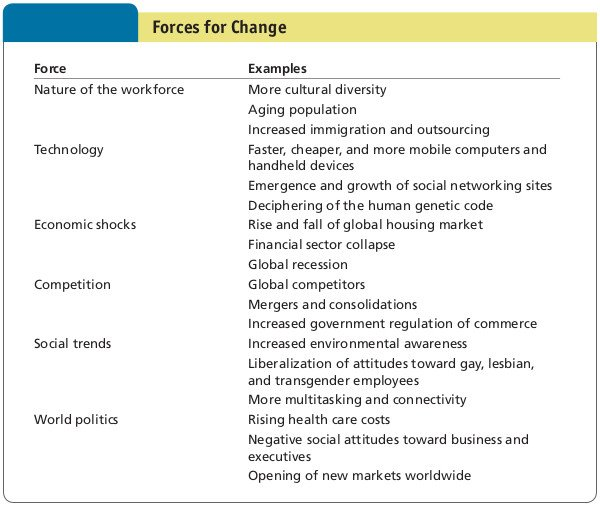
\includegraphics[scale=0.52]{./image/Change/Forces_for_Change.jpg}
	\caption{Forças para a Mudança \cite{book-7}}
\end{figure}
Empresas de todo tipo e dimensão estão a ser enfrentados com a questão de como podem assegurar o fornecimento de líderes com as competências, habilidades e visão estratégica adequadas para obter o sucesso. Ignorando a velha mentalidade de que certos indivíduos nascem para liderar, muitas empresas acreditam que a liderança pode ser desenvolvida numa forma pro-ativa e de forma sistemática. \cite{book-6}
\emptyline
A liderança assume um papel importante na mudança de cultura dentro das organizações e requer estar sempre em constante adaptação ao seu meio ambiente. Como sugere a liderança \textit{VUCA}, que representa Volatilidade, incerteza (uncertainty), complexidade e ambiguidade. Volatile porque não é estático esta e em constante mudança, incerteza na previsão do futuro, complexo com sistemas cada vez mais sofisticados que requer competências adequadas e ambíguo com problemas difícil de identificar, pouca informação de alternativas, sem se saber as consequências.
\begin{figure}[H]
	\centering
	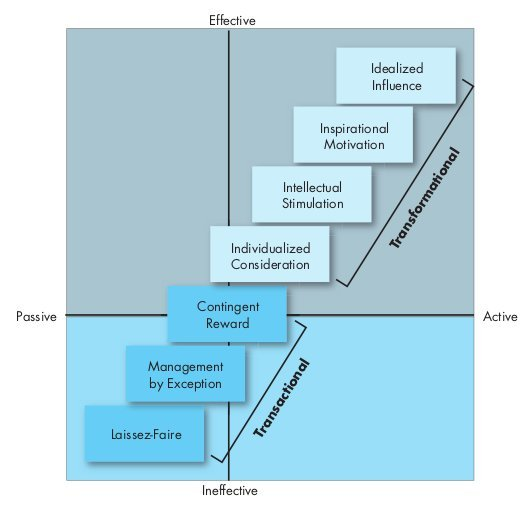
\includegraphics[scale=0.52]{./image/Leadership/Leadership_Models.jpg}
	\caption{Modelos da Liderança \cite{book-2}}
\end{figure}
Este trabalho esta focado no futuro do trabalho, gestão de carreira e marketing pessoal, no entanto abordar as matérias da gestão de mudança, a planeada (Modelo Kurt Lewin) e a emergente, os tipos de lideres, seus estilos e abordagens, também os modelos criados (Modelo Blake \& Mouton, Hersey \& Blanchard) são ferramentas úteis para nos orientar nos nossos comportamentos em diferentes contextos e determinar as atitudes a tomar com o nosso grupo ou equipa de forma a poder alcançar os objetivos e uma visão, ou seja garantir a sobrevivência e prosperidade da organização.
\begin{figure}[H]
	\centering
	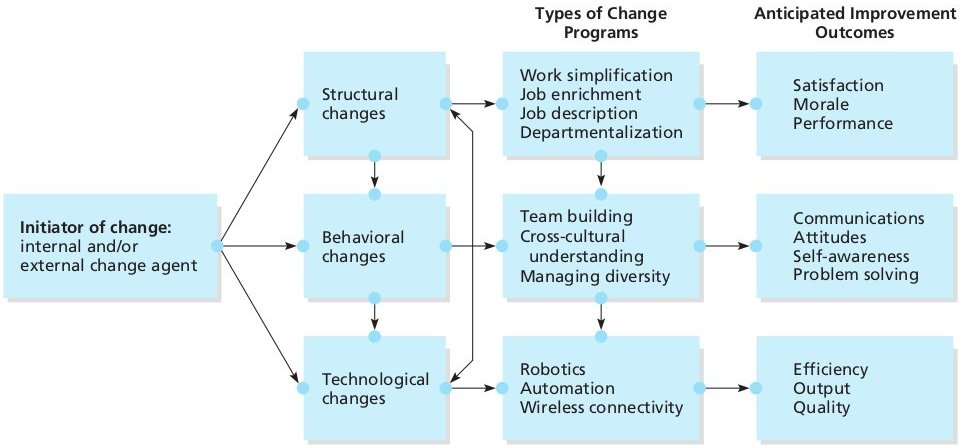
\includegraphics[scale=0.52]{./image/Change/Three_Change_Approaches.jpg}
	\caption{Três formas de mudar \cite{book-6}}
\end{figure}
